% !TeX TXS-program:compile = txs:///pdflatex/[--shell-escape]
\pdfoptionpdfminorversion=5
\documentclass[10pt, aspectratio=169, t ,hyperref={pdfpagelabels=false}]{beamer}
\usepackage{pgfpages}
%\setbeameroption{show notes on second screen=right}

\mode<presentation> {
    \usetheme{HHUD}
    \setbeamercovered{invisible}
}
\usepackage[ngerman]{babel}
\usepackage[utf8]{inputenc}
\usepackage{times}
\usepackage[T1]{fontenc}
\usepackage{amsmath}
\usepackage{tabularx} % tabularx Umgebung für mehr Kontrolle über Tabellen.
\usepackage{booktabs} % \toprule, \midrule, \bottomrule
\usepackage{multirow}
\usepackage{multicol}
\usepackage{longtable} % Große Tabellen gehen über mehrere Seiten.
\usepackage{subfigure}
\usepackage{graphicx}
\usepackage{hyperref}
\usepackage{xmpmulti}
\usepackage{siunitx}
\usepackage{tikz, pgfplots}
\usetikzlibrary{arrows,fit,calc,positioning,fadings}
\pgfplotsset{compat=1.18}
\usepackage{icomma}
\usepackage{csquotes}
\usepackage{listings}
\usepackage{minted}
\usepackage[backend=bibtex,style=verbose,url=false]{biblatex}
\bibliography{lit}
% If you want to exclude the appendix from the frame counter you have to use the appendixnumberbeamer package. But be aware that the current version causes a problem with the frame counter.
\usepackage{appendixnumberbeamer}

%% Die folgenden Zeilen können auskommentiert werden, um vor jedem Kapitel eine Gliederungsfolie einzufügen
% \AtBeginSection[] {
%   \begin{frame}<beamer>
%     \thispagestyle{empty}
%     \frametitle{Gliederung}
%     \vspace{-5mm}
%     \tableofcontents[currentsection]
%   \end{frame}
% }

\usebackgroundtemplate{
\includegraphics[width=\paperwidth]{fig/background_cd_2020}}

\newcommand{\backgroundNormal}{\usebackgroundtemplate{
    
\includegraphics[width=\paperwidth]{fig/background_cd_2020}}}
\newcommand{\backgroundTitle}{\usebackgroundtemplate{
    
\includegraphics[width=\paperwidth]{fig/background_heine}}}
\newcommand{\backgroundEmpty}{\usebackgroundtemplate{
    
\includegraphics[width=\paperwidth]{fig/background_empty}}}

\setlength{\leftmargini}{9pt}
\setbeamersize{text margin left=25pt,text margin right=25pt}
\setbeamertemplate{itemize/enumerate subbody end}{\vspace{.5\baselineskip}}

% % % % % % % % % %  CHANGE TOPIC AND AUTHOR INFORMATION HERE % % % % % % % % %
\newcommand{\abschluss}{Bachelor}                              % HIER UNZUTREFFENDES LÖSCHEN
\title{\abschluss{}arbeit:\\Entkopplung der Z3 Komponente in ProB mit ZeroMQ}                      % HIER DEN TITEL DER ARBEIT EINTRAGEN
\author{Silas A. Kraume}                                                       % HIER DEN NAMEN UND VORNAMEN EINTRAGEN
\date{13.02.2025}                                                                % HIER DAS PRÄSENTATIONSDATUM EINTRAGEN
% % % % % % % % % % % % % % % % % % % % % % % % % % % % % % % % % % % % % % % %
\institute{Institut für Informatik\\Heinrich-Heine-Universität Düsseldorf}
\subject{Informatik}

%
% Hier beginnt das Dokument
%
\begin{document}

\backgroundTitle
  \begin{frame}
    \thispagestyle{empty}
    \begin{columns}
    \column{0.4\paperwidth}
    {
    \footnotesize
    \color{hhuBlau}
    \put(20,-200){\insertdate}

    }
    \column{0.6\paperwidth}

    \color{hhuBlau}
    \LARGE \inserttitle\\[\baselineskip]

    \large \insertauthor
    \end{columns}
  \end{frame}
  \backgroundNormal

%   \begin{frame}
%     \thispagestyle{empty}
%     \frametitle{Gliederung}
%     Diese Gliederung ist optional und nicht unbedingt empfohlen (vor allem bei Präsentationen unter einer halben Stunde; löschen in master.tex – es ist auch jedem vollkommen klar, dass die grobe Struktur Einleitung, Methoden, Ergebnisse, Fazit ist; die Struktur erwähnt man kurz mündlich, solange man beim Titel-Slide ist)
%     \vspace{-5mm}
%     \tableofcontents
%   \end{frame}

  % % % % % % % % % % Ab hier werden die LaTeX-Dateien der einzelnen Abschnitte eingefügt % % % % % % % % % %

  \section{Einleitung}

\subsection{Foliengestaltung}

\begin{frame}{Motivation und Zielsetzung}
    \begin{figure}[!htp]
        \centering
        \resizebox{0.8\textwidth}{!}{
            \begin{tikzpicture}[
                    HOT/.style={rectangle, draw=red!60, fill=red!5, very thick, minimum size=40, align=center},
                    PB/.style={rectangle, draw=blue!60, fill=blue!5, very thick, minimum size=40, align=center},
                    COLD/.style={rectangle, draw=black!40, fill=black!3, very thick, minimum size=40, align=center},
                ]
                \begin{scope}
                    \node[PB]    (ProB)                             {ProB};
                    \node[HOT]    (C_Interface)       [right=of ProB] {C-Interface\\Z3-Solver};
                    \node[draw=none,fill=none,rectangle,above=0.5cm of ProB,xshift=-0.5cm,anchor=south west]
                    (Arch_A){Bestehende Architektur};

                    \draw[->, very thick] ([yshift=0.4cm]ProB.east)  to node[above,scale=1] {\tiny{constraint}} node[below,scale=1] {\tiny{posting}} ([yshift=0.4cm]C_Interface.west);
                    \draw[<-, very thick] ([yshift=-0.4cm]ProB.east) to node[below,scale=1] {\tiny{Solution}} ([yshift=-0.4cm]C_Interface.west);
                \end{scope}
                \node[draw,inner xsep=0.5cm, inner ysep=0.5cm,fit=(Arch_A) (ProB) (C_Interface)] (LeftScope){};
                \node[draw,dashed,inner xsep=0.2cm,inner ysep=0.2cm,fit=(ProB) (C_Interface)] (P0){};

                \begin{scope}[xshift=6.5cm]
                    \node[PB]    (ProB)        {ProB};
                    \node[HOT]    (C_Interface)       [right=of ProB] {C-Interface};
                    \node[HOT]    (Z3_Solver)       [right=of C_Interface] {Z3-Solver};
                    \node[COLD]    (Z3_Solver_G1)       [above=of Z3_Solver] {Z3-Solver};
                    \node[COLD]    (Z3_Solver_G2)       [below=of Z3_Solver] {Z3-Solver};
                    \node[draw=none,fill=none,rectangle,above=1cm of ProB,xshift=1cm,anchor=south west]
                    (Arch_B){Zielarchitektur};

                    \draw[->, very thick] ([yshift=0.4cm]ProB.east)  to node[above,scale=1] {\tiny{constraint}} node[below,scale=1] {\tiny{posting}} ([yshift=0.4cm]C_Interface.west);
                    \draw[<-, very thick] ([yshift=-0.4cm]ProB.east) to node[below,scale=1] {\tiny{Solution}} ([yshift=-0.4cm]C_Interface.west);
                    \draw[<->, very thick] (C_Interface) to node[below,scale=1] {\tiny{ZMQ}} (Z3_Solver);
                    \draw[<->, dashed, thick] (C_Interface.north east) to node[right,scale=1] {\tiny{ZMQ}} (Z3_Solver_G1.south west);
                    \draw[<->, dashed, thick] (C_Interface.south east) to node[right,scale=1] {\tiny{ZMQ}} (Z3_Solver_G2.north west);
                \end{scope}
                \node[draw,dashed,inner xsep=0.2cm,inner ysep=0.2cm,fit=(ProB) (C_Interface)] (P1){};
                \node[draw,dashed,inner xsep=0.2cm,inner ysep=0.2cm,fit=(Z3_Solver)] (P2){};
                \node[draw,dashed,inner xsep=0.2cm,inner ysep=0.2cm,fit=(Z3_Solver_G1)] (P3){};
                \node[draw,dashed,inner xsep=0.2cm,inner ysep=0.2cm,fit=(Z3_Solver_G2)] (P4){};
                \node[draw,inner xsep=0.5cm,inner ysep=0.5cm,fit=(ProB) (Z3_Solver_G1) (Z3_Solver_G2)] (RightScope){};

                \draw[->, double, thick, shorten <= 2pt, shorten >= 2pt] (LeftScope.east) -- (LeftScope-|RightScope.west);

                % \node at (0,-1.8) {\small Legende:};
                \node[PB, minimum width=0.4cm, minimum height=0.4cm] at (-0.4,-2.2) {};
                \node[right] at (0,-2.2) {\small ProB};
                \node[HOT, minimum width=0.4cm, minimum height=0.4cm] at (-0.4,-2.7) {};
                \node[right] at (0,-2.7) {\small Komponenten-Entkopplung};
                \node[draw,dashed, minimum width=0.4cm, minimum height=0.4cm] at (-0.4,-3.2) {};
                \node[right] at (0,-3.2) {\small Individuelle Prozesse};

            \end{tikzpicture}
        }
        % \caption{Die umgesetzte Architekturänderung.}
        % \label{fig:architecture}
    \end{figure}
\end{frame}

\begin{frame}{Hintergrundinformationen}
    \vspace{1em}
    \Large
    \begin{center}
        \begin{itemize}
            \item ProB: Animator, Model Checker und Constraint Solver für B-Methoden.
            \item Z3: Constraint Solver von Microsoft Research.
            \item ZeroMQ: Kommunikationsbibliothek für verteilte Systeme.
        \end{itemize}
    \end{center}
\end{frame}


  \section{Ergebnispräsentation}

\begin{frame}{Kommunikationsprotokoll}
  \vspace{1em}
%   \Large
  \begin{figure}[!ht]
    \centering
    \begin{tikzpicture}[scale=1.3, every node/.style={scale=1.3}]
        % Request box
        \node[above] at (2, 2.5) {\textbf{Request}};
        \draw[thick] (0, 2.5) rectangle (4, 0);
        \node[below] at (2, 2.5) {$F_\text{id}$};
        \draw[thick] (0, 2) -- (4, 2);
        \node[below] at (2, 2) {$F_\text{argument}(1)$};
        \draw[dashed] (0, 1.35) -- (4, 1.35);
        \node[below] at (2, 1.53) {$\vdots$};
        \draw[dashed] (0, 0.7) -- (4, 0.7);
        \node[below] at (2, 0.7) {$F_\text{argument}(n)$};
        \draw[decorate, decoration={brace, amplitude=10pt}] (4.1, 2) -- (4.1, 0)
            node[midway, right=16pt] {\text{zmsg\_t}};
        \draw[decorate, decoration={brace, amplitude=3pt}] (4.1, 2.5) -- (4.1, 2)
            node[midway, right=18pt] {\text{Integer}};
        % Response box
        \node[above] at (8.5, 2.5) {\textbf{Response}};
        \draw[thick] (6.5, 2.5) rectangle (10.5, 0);
        \node[below] at (8.5, 2.5) {$Status_\text{id}$};
        \draw[thick] (6.5, 2) -- (10.5, 2);
        \node[below] at (8.5, 2) {$F_\text{return\_value}(1)$};
        \draw[dashed] (6.5, 1.35) -- (10.5, 1.35);
        \node[below] at (8.5, 1.53) {$\vdots$};
        \draw[dashed] (6.5, 0.7) -- (10.5, 0.7);
        \node[below] at (8.5, 0.7) {$F_\text{return\_value}(n)$};
        \draw[decorate, decoration={brace, amplitude=10pt}] (6.4, 0) -- (6.4, 2);
        \draw[decorate, decoration={brace, amplitude=3pt}] (6.4, 2) -- (6.4, 2.5);

    \end{tikzpicture}
    % \caption{Das Kommunikationsprotokoll zwischen Client und Server.}
    % \label{fig:protocol}
  \end{figure}
\end{frame}

\begin{frame}{Struktur einer refaktorisierten Interfacefunktion}
    \begin{figure}[!htp]
        \centering
        \begin{tikzpicture}[scale=0.9, every node/.style={scale=0.9}]
            % Interfacefunktion
            \draw[thick] (0, 6.5) rectangle (5, 0);
            \draw[thick] (5, 6.5) -- node[below,sloped,pos=0.6]{\small \textbf{Interfacefunction}} (9, 6.5);
            % \node[above] at (1.6, 6.5) {\small \textbf{Interfacefunction}};
            \draw[thick,->,blue] (0.1, 6) -- (4.9, 6) node[above,midway,yshift=-2]{\tiny \textbf{Initial Request}};
            \node[below] at (2.5, 2) {\tiny $\vdots$};
            \draw[thick,<-,orange] (0.1, 0.8) -- (4.9, 0.8) node[below,midway,yshift=-2]{\tiny \textbf{Final Response}};

            \fill[black!10] (0.25, 5.5) rectangle (4.75, 3.3);
            \draw[] (0.25, 5.5) rectangle (4.75, 3.3);
            \draw[] (4.75, 5.5) -- node[below,sloped,pos=0.65]{\tiny \textbf{Helperfunction}} (8, 5.5);
            % \node[above] at (1.1, 5.4) {\tiny \textbf{Helperfunction}};
            \draw[thick,<-,orange] (0.5, 5.2) -- node[below,sloped,pos=0.3,yshift=2.5]{\tiny \text{Reply}} (4.5, 5.2);
            \draw[dashed,->,blue] (0.5, 4.8) -- (4.5, 4.8);
            \draw[dashed,<-,orange] (0.5, 4.5) -- (4.5, 4.5);
            \draw[] (0.6, 4.9) -- (0.4, 4.9) -- (0.4, 4.4) -- (0.6, 4.4);
            \draw[] (4.4, 4.9) -- (4.6, 4.9) -- (4.6, 4.4) -- (4.4, 4.4);
            \node[below] at (2.5, 4.6) {\tiny $\vdots$};
            \draw[thick,->,blue] (0.5, 3.6) -- node[above,sloped,pos=0.7,yshift=-2.5]{\tiny \text{Request}} (4.5, 3.6);

            \fill[black!10] (0.25, 3) rectangle (4.75, 2);
            \draw[] (0.25, 3) rectangle (4.75, 2);
            \draw[] (4.75, 3) -- node[below,sloped,pos=0.65]{\tiny \textbf{Helperfunction}} (8, 3);
            % \node[below] at (2.5, 3) {\tiny $\vdots$};


            % % Request box
            % \draw[thick] (0, 2.5) rectangle (4, 0);
            % \node[below] at (2, 2.5) {$F_\text{id}$};
            % \draw[thick] (0, 2) -- (4, 2);
            % \node[below] at (2, 2) {$F_\text{argument}(1)$};
            % \draw[dashed] (0, 1.35) -- (4, 1.35);
            % \node[below] at (2, 1.53) {$\vdots$};
            % \draw[dashed] (0, 0.7) -- (4, 0.7);
            % \node[below] at (2, 0.7) {$F_\text{argument}(n)$};
            % \draw[decorate, decoration={brace, amplitude=10pt}] (4.1, 2) -- (4.1, 0)
            %     node[midway, right=10pt] {\text{zmsg\_t}};
            % \draw[decorate, decoration={brace, amplitude=3pt}] (4.1, 2.5) -- (4.1, 2)
            %     node[midway, right=12pt] {\text{Integer}};

        \end{tikzpicture}
        % \caption{Die Modularität der Hilfsfunktionen innerhalb einer Interfacefunktion.}
        % \label{fig:help_modular}
    \end{figure}
\end{frame}

\begin{frame}{Logging}
    \vspace{2em}
    \Large
    \begin{enumerate}
        \item dient der verbesserten Nachvollziehbarkeit und Transparenz
        \item lässt sich über die Systemargumente steuern (\enquote{\texttt{-}\texttt{-}log})
        \item schreibt beispielsweise in \texttt{z3rver96485092.probz.log}
    \end{enumerate}
\end{frame}

\begin{frame}[fragile]{Softlock} % verbatim-Umgebungen sind fragil!
    \vspace{2em}
    \inputminted[linenos=false]{c++}{softlocka.cpp}
\end{frame}

\begin{frame}[fragile]{Softlock} % verbatim-Umgebungen sind fragil!
    \vspace{2em}
    \inputminted[linenos=false]{c++}{softlockb.cpp}
\end{frame}

\begin{frame}{Performance-Overhead}
    \begin{center}
        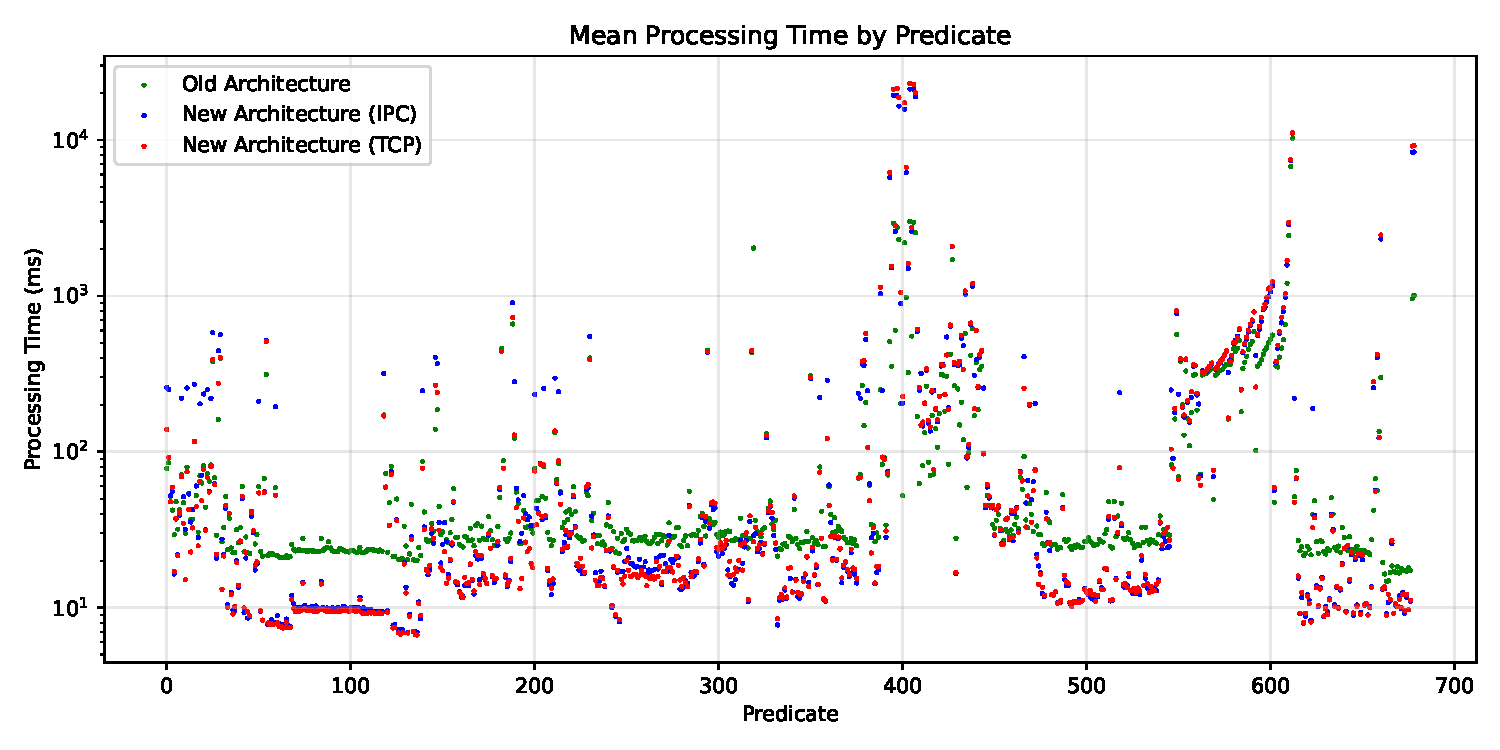
\includegraphics[width=0.85\textwidth]{../Thesis/PerformanceEvaluation/processingtime_small.pdf}
    \end{center}
\end{frame}


  \section{Fazit}

\begin{frame}{Fazit}
    \vspace{3em}
    \Large
    \begin{itemize}
        \item Die Restrukturierung des Systems konnte erfolgreich umgesetzt werden
        \item Es wurde eine unerwartete Laufzeitverbesserung erzielt
    \end{itemize}
\end{frame}


  \appendix

  \section{Anhang}
\begin{frame}{Anhang}
    Bild von successfull tests
    Messwert tabelle

    exceptions iwas
    evtl hilfsfunktion
\end{frame}


  % % % % % % % % % % Ende der eingefügten LaTeX-Dateien % % % % % % % % % %

\end{document}

%
% Hier endet das Dokument
%
